Pour solutionner ce problème, il faudra tout d'abord étudier le problème sur une application simplifiée (voir figure~\ref{model}) comprenant des liaisons entre modèles poblématiques et mettant bien en valeur l'intêret de ce stage. Ce modèle est
présenté dans le schéma ci dessous. L'application PROCOR a créer devra simuler l'intéraction entre un lit de débris et un bain de corium. Le lit de débris, comme le bai nde corium, aura deux états : un état à une couche
et un état à deux couches. On peut avoir des échanges internes entre chaque couche du composant, et l'on a aussi des échanges entre les composants du modèle. Ces intéractions ont été créé pour être problématiques et pour mettre
en valeur l'importance qu'à le couplage entre les composants d'une application PROCOR. 
\begin{figure}[h]
\centering
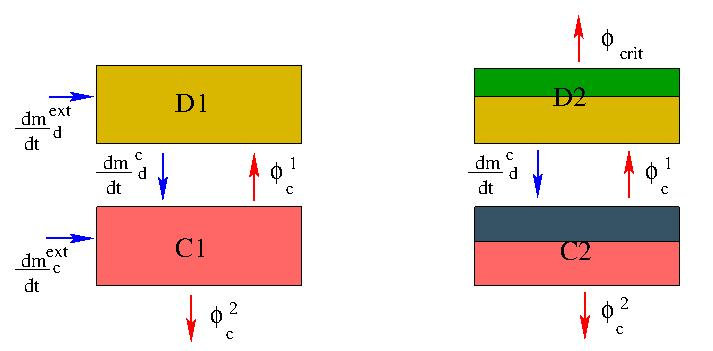
\includegraphics[scale=0.5]{model.jpeg}
\caption{Modèle simplifé : en haut le lit de débris, en bas le bain de corium. De gauche à droite, les deux états de chaque composant}
\label{model}
\end{figure}

Ensuite, une fois le problème bien compris sur le modèle simplifié, on pourra utiliser un schéma de prédicteur/correcteur pour améliorer le couplage sur la boucle temporelle externe des différents composants d'une application
PROCOR. Ce schéma permettra de simuler le déroulement de l'application et ainsi d'optimiser l'application en estimant l'erreur commise en fonction du couplage effectué. On pourra aussi, pour automatiser le couplage, essayer
de construire une architecture de code en programmation objet en Java permettant cette automatisation pour faciliter la construction d'application PROCOR.\\ 

Si ceci est terminé avant la fin du stage, il serait aussi interessant d'étudier le comportement interne des composants du modèle et essayer de synchroniser leur paramètre avec d'autres composants par le biais de 
"Message Passing". Ainsi si par exemple, le lit de débris se liquifie à un instant à l'intérieur de la boucle temporelle, un message sera envoyé aux autres composants pour prévenir d'un changement d'état. On pourra 
ainsi améliorer la robustesse et la précision de la simulation. Le résultat vraiment attendu du stage est l'implantation du schéma prédicteur/correcteur, le codage du "Message Passing" ne sera fait que si il reste du temps
à la fin du stage.  